%Modified from a template provided by Jennifer Pan, August 2011

\documentclass[10pt,letter]{article}
	% basic article document class
	% use percent signs to make comments to yourself -- they will not show up.
\usepackage{pdfsync}
\usepackage{amsmath}
\usepackage{amssymb}
\usepackage{amsthm}
\usepackage[makeroom]{cancel}
	% packages that allow mathematical formatting
\usepackage{mathrsfs}

\usepackage{graphicx}
	% package that allows you to include graphics
\graphicspath{ {./images/} }


\usepackage{subcaption}

\usepackage{setspace}
	% package that allows you to change spacing

\onehalfspacing
	% text become 1.5 spaced

\usepackage{fullpage}
% package that specifies normal margins

\usepackage[parfill]{parskip}

\newtheorem*{thm}{Theorem}
\newtheorem{nthm}{Theorem}
\newtheorem{lem}{Lemma}

\begin{document}
	% line of code telling latex that your document is beginning

\title{Problem Set 5}

\author{Katherine Cheng, Richard Davis, Marty Keil}

% \date{Friday April 10, 2015}
	% Note: when you omit this command, the current date is automatically included
 
\maketitle 
	% tells latex to follow your header (e.g., title, author) commands.

\section*{Problem One} Richard Davis submitted these (suid: rldavis).

\section*{Problem Two} Richard Davis submitted these (suid: rldavis).

\section*{Problem Three} 

\paragraph{i.} \texttt{a*b*}
\paragraph{ii.} \texttt{b?(ab?)*}
\paragraph{iii.} \texttt{((yd)*|(dy)*|(yyd(yd)*d)*|(ddy(dy)*y)*)*}
\paragraph{iv.} \texttt{epsilon | a | ( b | aa | ab(a|b) ) (a|b)*}

\section*{Problem Four: Powerset of $\Sigma^*$}
If $\Sigma$ is an alphabet, then $\Sigma^*$ is the set of all strings composed from letters in $\Sigma$. The powerset of $\Sigma^*$ is the set of all $\Sigma^*$'s subsets. In other words, the powerset is the set of all possible languages in the alphabet $\Sigma$. 

\section*{Problem Five: Cardinalities and Concatenations}
Prove or disprove: if $L$ is a language and $k \ge 1$, then $|L^k| = |L|^k$. (As a special case, the language $L^0$ is defined to be $\{\varepsilon\}$.)

\begin{thm}
If $L$ is a language and $k \ge 1$, then $|L^k| = |L|^k$.
\end{thm}

The definition of language concatenation is: If $L_1$ and $L_2$ are languages over $\Sigma$, the concatention of $L_1$ and $L_2$ is the language $L_1L_2$ defined as $L_1L_2 = \{ wx \ | \ w \in L_1 \text{ and } x \in L_2 \}$. From this it follows that the k-fold concatenation of $L$ can be represented by every possible k-tuple of the strings in the language L concatenated together.

We can construct the k-fold concatenation of some language $L$ by finding every possible k-combination of strings in $L$. This is an ordered samples with replacement problem. There are $|L|$ possible choices for the first string, $|L|$ possible choices for the second string, and so on until the kth string. In other words, there are $|L|^k$ possible k-combinations of the strings in $L$. 

\section*{Problem Six: Finite and Cofinite Languages}

\paragraph{i.} 

Assume $L$ is finite. $L$ is a language over $\Sigma$, which means that $L$ is a set of strings over $\Sigma$. Since $L$ is finite, we know that $L$ is a finite set of strings. Let $k$ be $|L|$, the number of strings in $L$.

We can create an NFA $N$ comprised of a start state, and $k$ $\epsilon$ transitions from the start state to $k$ distinct states. Each of these $k$ states could then point to a set of states and transitions corresponding to one string in $L$, where the final state is an accepting state. Thus, each string in $L$ would be in the set of strings that N accepts. This means that each string in $L$ is represented in the language of $N$, $L(N)$.

We know from lecture that a language $L$ is regular iff there is some NFA $N$ such that $L(N) = L$.

We have shown that there exists an NFA $N$ such that $L(N) = L$. Therefore, $L$ is a regular language.

\paragraph{ii.} Any cofinite language has a complement that is finite. If the complement is finite it is a regular language and has a DFA , as shown in part i. This DFA has a finite number states, some of which are accepting states. If the cofinite language is a complement of this DFA then a new DFA representing the cofiinite language can always be formed as shown in lecture.  In this new DFA all accepting states are reversed for the finite DFA complement. Therefore the co-finite is a regular language, since there exists a DFA D such that $\mathscr{L}$ (D) = L . 

\section*{Problem Seven: State Elimination}

\paragraph{i.} After bypassing states $q1$ and $q2$ we get the following DFA:\\

\begin{figure}[h]
\centering
  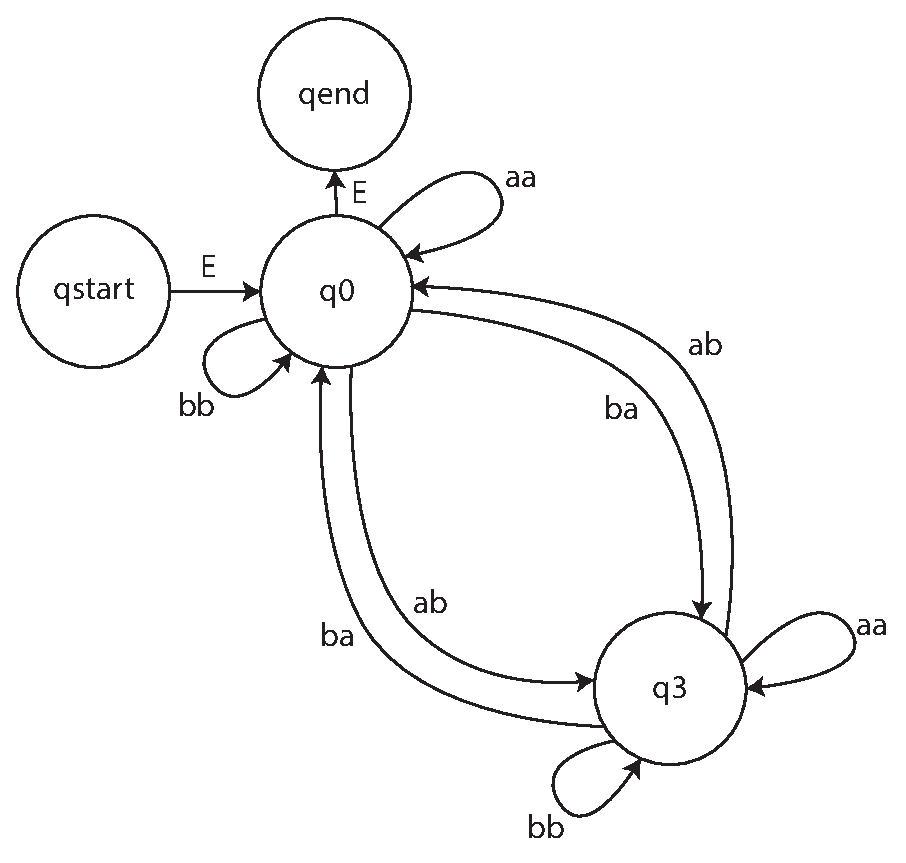
\includegraphics[width=0.45\linewidth]{7i.eps}
  \caption{DFA after bypassing q1 and q2}
  \label{fig:7i}
\end{figure}

\paragraph{ii.} We got $( (aa|bb) | (ab|ba) (aa|bb)^{*} (ab|ba))^{*}$.

\section*{Problem Eight: Derivatives of Regular Languages}

\paragraph{i.} We are taking the derivative of $a$ over the language $L$. To construct a DFA for the derivative, first create a new state $q_{ns}$ and make this the new start state for the DFA. Second, take the first transition from the old start state $q_s$ using character $a$ to some state we will call $q_0$. If there is no transition on a, delete the entire DFA. Otherwise, follow the transition to the next state that we will call $q_0$. This state $q_0$ may or may not be $q_s$. This is no matter. If $q_0$ exists, create a transition from the new start state $q_{ns}$ to the state $q_0$. This creates a new DFA, DFA$_{new}$, that only accepts strings in the language that start with a. To finish DFA$_{new}$, make $q_0$ the new start state. 

\paragraph{ii.} 
\begin{thm} DFA$_{new}$ accepts a string $w \in \Sigma^* \text{ if and only if } w \in \partial_a L$. 
\end{thm}

\begin{proof} To prove this, we must first prove that if DFA$_{new}$ accepts a string $w \in \Sigma^*$ then $w \in \partial_a L$. Second, we must prove that if $w \in \partial_a L$ then DFA$_{new}$ accepts it.

We prove the first statement by contradiction. Assume for the sake of contradiction that DFA$_{new}$ accepts some string $w \in \Sigma^*$ and $w \not \in \partial_a L$. If $w \not \in \partial_a L$ then by definition the original string $w$ did not start with the letter a. However, DFA$_{new}$ was constructed in a way so that only strings that originally had at least one letter a at the front could be accepted. This is a contradiction so our assumption must be false.

We prove the second statement by contradiction as well. Assume for the sake of contradiction that $w \in \partial_a L$ and DFA$_{new}$ does not accept it. By definition, if $w \in partial_a L$ this means that the original string must have started with at least one $a$. However, DFA$_{new}$ was constructed so that it can only accept strings that originally started with at least one $a$. This is a contradiction so our assumption must be false.

Thus we prove that DFA$_{new}$ accepts a string $w \in \Sigma^* \text{ if and only if } w \in \partial_a L$. 

\section*{Problem Nine: Why the Extra State?} 
One of the languages that this does not work for is defined by the regular expression \texttt{a*b}. This can be represented by the NFA that looks like this:

\begin{figure}[h]
\centering
  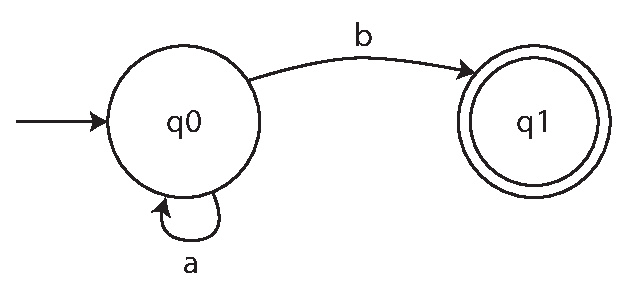
\includegraphics[width=0.45\linewidth]{9i.eps}
  \caption{NFA for \texttt{a*b}}
  \label{fig:9i}
\end{figure}

If we try to make an epsilon transition back to the start state and make that an accepting state, we end up with the following NFA.

\begin{figure}[h]
\centering
  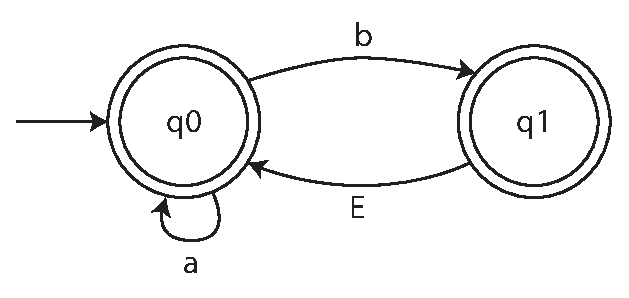
\includegraphics[width=0.45\linewidth]{9ii.eps}
  \caption{Wrong NFA for \texttt{a*b}}
  \label{fig:9ii}
\end{figure}

This ends up accepting, for example, the string ``a,'' which is not a part of the language.

% \Section*{Appendix: Referencing Equations}
% \begin{equation} \label{eq:divbyzero}
%   \frac {1} {0}
% \end{equation}

% This references \ref{eq:divbyzero}.

% \section*{Appendix: Figures in Text}
% Below are two different ways of placing figures side by side in text. The first method creates two sub-figures within a single figure. The second method creates two separate figures.

% \begin{figure}
% \centering
% \begin{minipage}{.5\textwidth}
%   \centering
%   \includegraphics[width=.8\linewidth]{hw3_8_1.eps}
%   \captionof{figure}{A figure}
%   \label{fig:q8_test1}
% \end{minipage}%
% \begin{minipage}{.5\textwidth}
%   \centering
%   \includegraphics[width=.8\linewidth]{hw3_8_1.eps}
%   \captionof{figure}{Another figure}
%   \label{fig:q8_test2}
% \end{minipage}
% \end{figure}


% \begin{figure}[h]
%   \centering

%   \begin{subfigure}[b]{0.3\textwidth}
%     \includegraphics[width=\textwidth]{hw3_8_1.eps}
%     \caption{A cycle with length $k+1$}
%     \label{fig:q8_cycle:a}
%   \end{subfigure}% 
%   \qquad
%   \begin{subfigure}[b]{0.3\textwidth}
%     \includegraphics[width=\textwidth]{hw3_8_1.eps}
%     \caption{A cycle with length $k+1$}
%     \label{fig:q8_cycle:b}
%   \end{subfigure}%  

%   \caption{Placeholder}
%   \label{fig:q8}
% \end{figure}

\end{document}
	% line of code telling latex that your document is ending. If you leave this out, you'll get an error

%%% Local Variables:
%%% mode: latex
%%% TeX-master: t
%%% End:
